\documentclass[a4paper,12pt,twocolumn]{article}
\date{ }
\title{\textbf{Predicción del precio del Bitcoin mediante ventanas móviles y un ensamble de estimadores por Modelos Lineales modelados a través de Bagging con Árboles de Regresión.}}
\author{Vanessa Alcalde, Pablo Martinez Angerosa}
\usepackage[spanish]{babel}
\usepackage{graphicx}
\usepackage[tight]{subfigure}
\renewcommand{\figurename}{Figura}
\newtheorem{dfn}{Definición}
\renewcommand{\labelenumi}{P.\theenumi}
\renewcommand{\abstractname}{Resumen}
\renewcommand{\refname}{Bibliografía}
\renewcommand{\tablename}{Tabla} 
\usepackage{booktabs,xcolor,siunitx,amsmath }
\definecolor{lightgray}{gray}{0.9}

\begin{document}


\setlength{\columnsep}{0.8cm}
% now make the abstract span both columns
\twocolumn[
\maketitle

\begin{abstract}{

En la actualidad existen diversas investigaciones que analizan la composición del precio del Bitcoin y proponen técnicas de predicción del mismo basadas en Modelos Lineales, utilizando variables explicativas de rezagos del precio y el volumen del Bitcoin. Aquí presentamos una investigación que propone un sistema de ventanas móviles el cual genera un ensamble de estimadores mediante Modelos Lineales, cuyas predicciones son consideradas como opiniones expertas, y se utilizaron diversas técnicas (Ensamble de Modelos Lineales, Bagging con Árboles de Regresión y Redes Neuronales) para sintetizar estas opiniones en una predicción. Los resultados obtenidos muestran que bajo esta perspectiva, la técnica de Bagging obtiene un rendimiento ampliamente mayor que los modelos propuestos originalmente.
\vspace{1.0cm}} 
\end{abstract}
]

\vspace{1.0cm}


\section{Introducción}
Bitcoin, una criptomoneda digital, presentada en su inicio en foros especializados de criptografía \cite{Satoshi}, esta actualmente siendo integrada y aceptada por los principales actores del mundo de las finanzas. Considerándose esta situación, por muchos expertos en el tema, como la consolidación definitiva de esta moneda la cual se dirige hacia un futuro brillante. 

En la actualidad existen diversas investigaciones que analizan la composición del precio del Bitcoin y proponen técnicas de predicción del mismo \cite{mainDriversBitcoin}. Aunque hay matices de propuestas, el entendimiento del precio del Bitcoin como un paseo aleatorio, donde la historia del propio precio no tiene incidencia en su predicción posterior, es de común acuerdo entre las investigaciones. Esto conlleva a enfrentar este problema de predicción desde otra perspectiva a la de Series Temporales. Para esto se han investigado diversas metodologías dentro del enfoque de aprendizaje automático. En la gran mayoría de las investigaciones el algoritmo recomendado para la predicción del precio del Bitcoin es Modelos Lineales  \cite{regression_for_bitcoin_price}, basado principalmente en variables explicativas de rezagos del precio y el volumen del Bitcoin  \cite{forecastinBitcoinClosing}.  

El objetivo de esta investigación es proponer alternativas a las investigaciones realizadas actualmente sobre la predicción del precio del Bitcoin que logren mejorar el rendimiento de estas propuestas. 

Para esto se utilizó un sistema de ventanas móviles el cual genera un ensamble de estimadores mediante Modelos Lineales, que son consideradas como opiniones expertas, y se proponen diversas técnicas para sintetizar estas opiniones en una sola predicción. El modelo propuesto en esta investigación logra duplicar el rendimiento de las técnicas recomendadas en la literatura existente. Es de destacar que los realizadores de esta investigación han logrado generar algoritmos automáticos de compra-venta de Bitcoin  basados en los estimadores propuestos que logran en un  intervalo de corto plazo doblar la inversión inicial.  


A continuación, en la segunda sección de esta investigación detallamos la obtención y tratamiento de los datos, en la tercera sección describimos los modelos utilizados y el procedimiento, en la cuarta sección presentamos los resultados y finalmente en la quinta sección mostramos las conclusiones de esta investigación y posibles trabajos a futuro.



\section{Datos}
\subsection{Descripción de los datos}

Para la construcción de la base de datos utilizamos los datos por hora del precio de  $Cierre$ y $Volumen$ de transacciones de Bitcoin, provistos por Binance\footnote{https://www.binance.com} que es una casa de cambio digital la cual es considerada la plataforma de intercambio con el nivel de volumen comercial más grande del mundo. 

Binance cuenta con una API\footnote{Interfaz de Programación de Aplicaciones} en distintos lenguajes de programación, desde la cual es posible acceder de forma gratuita a los registros en tiempo real de las fluctuaciones del precio del Bitcoin así como también a los registros históricos de esta criptomoneda. Para esta investigación se generó una cuenta de usuario en Binance y se utilizó la API provista en Python\footnote{https://python-binance.readthedocs.io} para descargar los registros históricos por hora en dólares americanos (USD) de Bitcoin(BTC). 


\subsection{Preparación de los datos}

La base de datos contiene 8717 registros comenzando en el día $12/12/2019$ a las 08:00:00h hasta el $10/12/2020$ a la 01:00:00h. En la Figura~\ref{priceClose} se muestran los datos del $Cierre$ del Bitcoin como Serie Temporal en este intervalo de tiempo. 

\begin{figure*}[!hbt]
\centering
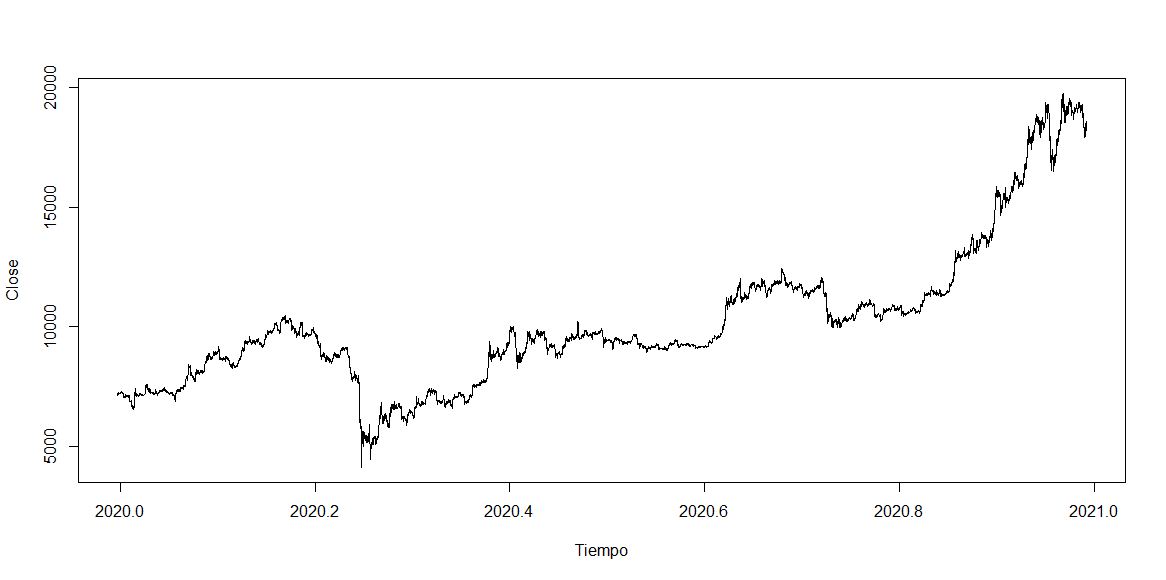
\includegraphics[width=1\textwidth]{serie}
\caption{Serie de Tiempo del precio del $Cierre$ por hora del Bitcoin desde el día $12/12/2019$ a las 08:00:00h hasta el $10/12/2020$ a la 01:00:00h.}
\label{priceClose}
\end{figure*}


La base se estructuró de modo de tener un conjunto de entradas $X$ y salidas $Y$ con una dependencia temporal. La variable de predicción $Y$ corresponde al $Cierre$ del precio del Bitcoin en el tiempo $n$. Las entradas correspondientes a $X$ se encuentran en diversos momentos del pasado. 

La variable $Volumen$ corresponde al tiempo $n-1$ ya que es información que no existe a la hora de predecir el momento $n$.

Se crearon variables de rezagos llamadas $lag$, para el precio de $Cierre$ y $Volumen$ de Bitcoin. Los números utilizados para nombrar las variables de rezago, representan el tiempo del pasado. Por ejemplo la variable $closeLag3$ representa el precio del $Cierre$ del Bitcoin 3 horas previas al momento $n$~\cite{forecastinBitcoinClosing}.  

Dada la experiencia previa obtenida a partir de investigaciones y la literatura las variables utilizadas son los cinco primeros rezagos del precio del $Close$ y del $Volumen$ del Bitcoin. En la base de datos estas variables son definidas como $closeLag1$, $closeLag2$, $closeLag3$, $closeLag4$, $closeLag5$, $volLag1$, $volLag2$, $volLag3$, $volLag4$ y $volLag5$, respectivamente.

\section{Los modelos}


\subsection{Metodología}

En esta sección presentamos las cuatro técnicas utilizadas que incluyen Modelos Lineales, Métodos de Ensamble de Modelos, Bagging basado en Árboles de Decisión y Redes Neuronales.

Un modelo de regresión lineal múltiple (\ref{ecuacionML}) es un Modelo Lineal en los parámetros en el cual la variable de respuesta, $Y$, es determinada por un conjunto de variables independientes, las variables explicativas (matriz $X$). Se busca el hiperplano que mejor ajuste a los datos. Los parámetros $\beta_i$ para el modelo se obtienen por mínimos cuadrados.

\begin{equation}
y_{i}=\beta_{0}+\beta_{1} x_{i}+\beta_{2} x_{i}+\cdots+\beta_{d} x_{i}+\epsilon_{i}
\label{ecuacionML}
\end{equation}

Los Métodos de Ensamble de Modelos son útiles para mejorar el rendimiento de los modelos de aprendizaje automático al mejorar su precisión. Se construyen varios modelos y se combinan las predicciones resultantes mediante su promedio. Este promedio de errores produce mejores predicciones generalizando el carácter particular de cada uno de estos modelos.

Un árbol de decisión es una división recursiva del espacio de variables explicativas en una estructura en forma de árbol, cada nodo interior contiene una pregunta sobre una variable de entrada y cada nodo terminal una decisión. Estos pueden ser utilizados en problemas de regresión y clasificación, en nuestro caso la variable explicada es continua por lo que trabajamos con árboles de regresión.  

Los árboles CART (Classification And Regression Tree) se construyen dividiendo el conjunto de valores posibles de $X_1,X_2,...,X_p$ en $J$ regiones disjuntas $R_1, R_2,..., R_J$. En el caso de un árbol de regresión, para cada observación en la región $R_j$ se predice el valor medio de las respuestas.

Para llevar a cabo la construcción del árbol se comienza con un conjunto de datos de entrenamiento, el cual es segmentado mediante particiones binarias. Se crean regiones $R_1, R_2,..., R_J$ de manera que se minimice la Ecuación (\ref{ecuacionTree}).


\begin{equation}
\sum_{j=1}^{J} \sum_{i \in R_{j}}\left(y_{i}-\hat{y}_{R_{j}}\right)^{2}
\label{ecuacionTree}
\end{equation}


Donde $\hat{y}_{R_{j}}$ es la respuesta media para las observaciones del conjunto de entrenamiento en la región j-ésima~\cite{libroCurso}.

Una vez que se encuentra la mejor partición, se separan los datos en las regiones resultantes y se repite el proceso. Este proceso termina cuando se satisface algún criterio de parada.

El método Bagging (Bootstrap Aggregating) es un procedimiento para reducir la varianza de un modelo de aprendizaje automático~\cite{libroCurso}.

Se divide el conjunto de datos en entrenamiento $L$ y testeo $T$, se toma una muestra bootstrap $L_b$ de $L$ y se construye un estimador usando $L_b$. Se repite el procedimiento $B$ veces. Luego a cada dato de $T$ se le asigna el promedio de las respuestas de los estimadores construidos en el paso anterior (para el caso de un modelo de regresión). La proporción de veces que la clase estimada difiere de la verdadera es el error Bagging. Luego puede repetirse la división de los datos en $L$ y $T$ varias veces y calcular los errores promedio.

Bagging puede ser utilizado para Árboles de decisión, para esto se construyen $B$ árboles con conjunto de entrenamiento obtenido mediante una muestra bootstrap del conjunto de entrenamiento original, luego se hace un promedio de las predicciones resultantes. Estos árboles tienen varianza grande pero sesgo bajo ya que no se podan. Al promediarlos se reduce la varianza y por lo tanto se mejora la precisión de las predicciones.

Las Redes Neuronales son un modelado matemático que homologa el comportamiento de una neurona biológica. El objetivo de su diseño es emular al cerebro humano. Básicamente se basa en una red de neuronas conectadas que reciben un estímulo de entrada y producen una salida.   

En su modelado matemático se construyen combinaciones lineales de las entradas y se obtiene la salida como una función no lineal de estas. 

En la Ecuación (\ref{ecuacionRedes}) se muestra el modelado de una red neuronal con una capa de entrada, una capa oculta y una salida. Donde $i$, $j$ son los índices correspondientes a la capa de entrada y oculta respectivamente, $w$ corresponde a los pesos de cada neurona y $f(.)$ a la función de activación.

\begin{equation}
g_{k}(x)=f \underbrace{(\sum_{j=1}^{n_{H}} w_{k j} f \underbrace{\left(\sum_{i=1}^{d} w_{j i} x_{i}+w_{j 0}\right)}_{\text {net }_{j}}+w_{k 0})}_{\text {net }_{k}}
\label{ecuacionRedes}
\end{equation}

El procedimiento para encontrar los pesos que configuren el mejor modelo consiste en primero multiplicar cada dato de entrada por un peso y los valores ponderados se combinan linealmente. Posteriormente se aplica una función de activación no lineal. El valor de salida es comparado con el valor objetivo. La diferencia de error que se produce es utilizada para actualizar los pesos y se itera hasta obtener el criterio deseado de parada. Actualmente el algoritmo más utilizado para esto es el de Backpropagation. Esta arquitectura crece en complejidad pero el algoritmo y los procesos son siempre los mismos. 

\begin{equation}
(min)RMSE=\sqrt{\frac{1}{N} \sum_{i=1}^{N}\left(y_{i}-f_{i}\right)^{2}}
\label{remseequation}
\end{equation}

Para evaluar el rendimiento de los distintos modelos de predicción se utilizó la medida de error RMSE como se ve en la Ecuación (\ref{remseequation}) donde $y_i$ representa las predicciones y $f_i$ los valores reales. Se busca minimizar el RMSE.

\subsection{Proceso}

En primer lugar, el conjunto de datos se dividió aleatoriamente, en una muestra de entrenamiento del $70\%$ y una muestra de testeo del $30\%$ donde se busca generalizar el comportamiento del precio del Bitcoin en ambas muestras.

El primer objetivo fue recrear la predicción del precio del Bitcoin mediante la estrategia de Modelos Lineales propuestas en la literatura e investigaciones anteriores. 

En la Figura \ref{diagramLinearRegression} se muestra el diagrama del proceso. En este caso para encontrar el modelo con mejor rendimiento se construyó un algoritmo de fuerza bruta que evalúa secuencialmente una a una todas las posibles combinaciones de las variables seleccionadas (cinco primeros rezagos de $Close$ y $Volumen$ del precio del Bitcoin) comparando el RMSE generado por cada una de estas combinaciones con la muestra de testeo. El modelo seleccionado es aquel con el menor RMSE. El orden de todas las combinaciones es de $2^n - 1$ para $n$ opciones de variables. En este caso contamos con $1023$ posibles modelos.


\begin{figure}[!hbt]
\centering
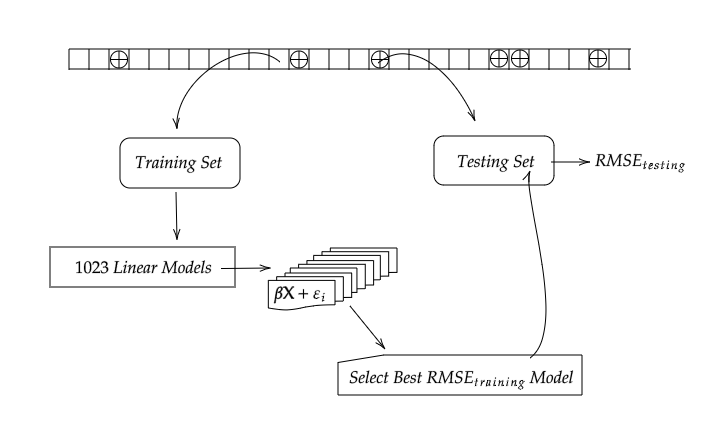
\includegraphics[width=0.5\textwidth]{diagramLinearRegression}
\caption{Diagrama del proceso de selección del Modelo Lineal con menor RMSE con respecto a la muestra de testeo a partir de un ensamble de $1023$ posibles modelos generados desde las combinaciones obtenidas de los cinco primeros rezagos de $Close$ y $Volumen$ del precio del Bitcoin.}
\label{diagramLinearRegression}
\end{figure}

En la búsqueda de nuevas propuestas de predicción, mediante la prueba y el error y otras sugerencias de la literatura, decidimos primariamente cambiar el enfoque estático de generación de muestras de entrenamiento y testeo hacia un enfoque dinámico mediante el concepto de ventanas móviles \cite{forecastinBitcoinClosing}. 

El concepto de ventanas móviles consiste en generar una ventana de entrenamiento, con una memoria de corto plazo, de un ancho de $w$ rezagos de tiempo para predecir el precio del Bitcoin en el momento $n$. Es decir, para predecir el precio en el momento $n$ se genera una ventana de $w$ rezagos  desde el momento $n-1$ hasta el momento $n-w-1$. En esta investigación se utiliza una ventana móvil de 25 rezagos, cuyo ancho es producto de la experimentación y recomendaciones en la literatura. 

El siguiente paso fue utilizar el concepto previamente descripto para Modelos Lineales pero en las ventanas móviles de corto plazo. Es decir, que para cada momento $n$ que se quiere predecir se genera un ensamble de $1023$ Modelos Lineales, a partir de todas las combinaciones de las variables seleccionadas, ajustados desde la muestra de entrenamiento que ahora es dinámica. Esta muestra de entrenamiento se actualiza por cada movimiento de la ventana. En este punto surgieron hallazgos importantes que dirigieron el rumbo de esta investigación. 

Un primer descubrimiento fue notar que la linealidad en cada una de las ventanas móviles era extremadamente fuerte ya que el RMSE obtenido con las mismas muestras de entrenamiento de cada ventana era considerablemente bajo y a medida que aumentábamos el $w$ de la ventana el RMSE aumentaba. Esto fue un indicio de que utilizar Modelos Lineales sobre el concepto de ventanas móviles es una buena opción ya que la linealidad en el corto plazo es fuerte.

Otro punto importante para el desarrollo de esta investigación fue el descubrimiento de que entre las $1023$ predicciones obtenidas por los modelos lineales en cada ventana en un  $76.15\%$ de los casos al menos uno de los modelos realizaba una estimación casi perfecta en un intervalo $\pm 5$ dólares. 

En la Figura \ref{muestras} se puede observar como en una muestra aleatoria de cuatro momentos de la base, en las primeras tres muestras el precio de $Close$ es contemplado en al menos una de las $1023$ predicciones. En la muestra $4$ se observa como ninguna de estas estimaciones logra predecir con una exactitud de $\pm 5$ dólares este precio. Este comportamiento se mantiene durante toda la base.

\begin{figure}[!htb]
\centering
\subfigure[Muestra 1.]
{ 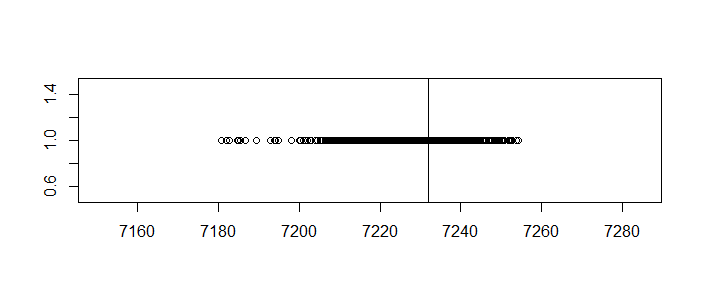
\includegraphics[width=5.0cm]{muestra1}
\label{muestra1}
}\\
\subfigure[Muestra 2.]
{ 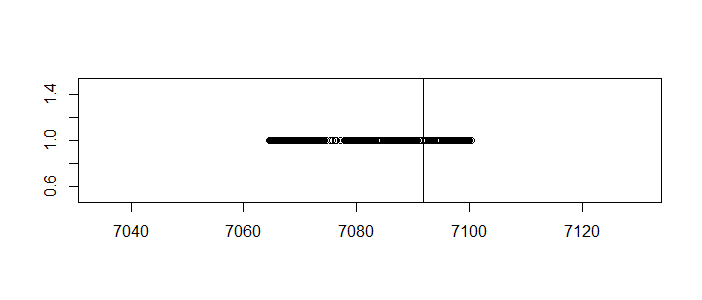
\includegraphics[width=5.0cm]{muestra2}
\label{muestra2}
}\hfill
\subfigure[Muestra 3.]
{ 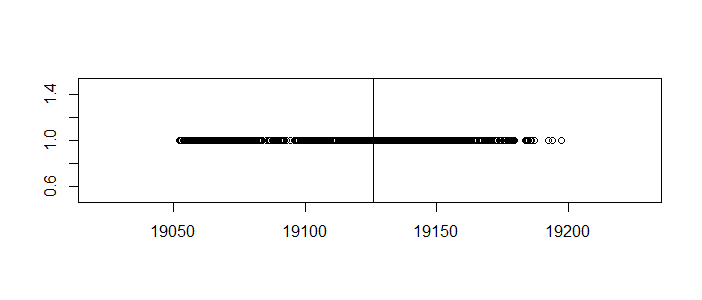
\includegraphics[width=5.0cm]{muestra3}
\label{muestra3}
}\hfill
\subfigure[Muestra 4.]
{ 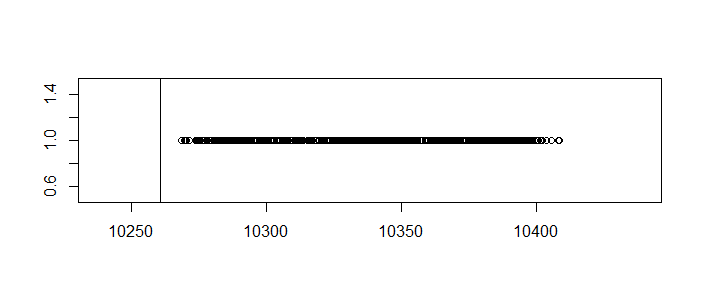
\includegraphics[width=5.0cm]{muestra4}
\label{muestra4}
}
\caption{Muestra aleatoria de cuatro momentos de la base y las $1023$ predicciones del precio de $Close$ generadas a partir de una ventana de $25$ rezagos para cada momento por Modelos Lineales. En cada una de las figuras se muestra con una línea vertical el precio de $Close$ real para cada momento y las predicciones se marcan con círculos.}
\label{muestras}
\end{figure}
%

De aquí en adelante la estrategia a seguir es  encontrar posibles patrones entre los precios estimados por cada uno de los $1023$ modelos y el precio real de $Close$ del Bitcoin en cada ventana móvil. Surgen las siguientes preguntas: cuando varios modelos estiman el mismo precio ¿hay una relación con el precio real?; ¿existe una relación cada vez que los primeros diez modelos predicen un precio muy cercano en sus predicciones y el precio real del $Close$?; etc. Los posibles patrones a encontrar entre este ensamble de predicciones y el precio real son muchos, entonces nuestra pregunta fundamental a responder es ¿existe algún patrón entre las $1023$ predicciones por ventana de rezagos y el precio real del Bitcoin?

Para enfrentar este nuevo enfoque creamos una nueva base de datos donde se mantiene la temporalidad de la base anterior pero se cambian las variables explicativas de cada fila. En esta nueva versión de la base de datos cada una de las filas, que representan el momento $n$ del precio del $Close$ del Bitcoin, está compuesta por un ensamble de $1023$ variables que mantienen en orden estricto las predicciones generadas por los $1023$ Modelos Lineales ajustados, a partir de las combinaciones de las variables anteriores (cinco primeros rezagos del precio de $Close$ y $Volumen$ del Bitcoin), en cada ventana correspondiente al momento $n$ de un ancho de $w$ rezagos.

En la Figura \ref{histograma} estudiamos el comportamiento de cada uno de los $1023$ modelos a lo largo de toda la base. El eje de abscisas representa en orden estricto cada uno de los modelos. El eje de las ordenadas indica la frecuencia absoluta con la que cada modelo correspondiente acierta en un intervalo de $\pm 5$ dólares durante el recorrido de la base. Podemos observar que existe un umbral mínimo que logran todos los modelos de $351$ ($4.03\%$) aciertos. Es decir, en todo el recorrido de la base cada uno de los modelos acertó al menos $351$ veces el precio del $Close$ del Bitcoin en el intervalo de $\pm 5$ dólares. También podemos observar que existen tres bandas de umbrales claros que se diferencian entre los modelos, el primer umbral de los primeros $250$ modelos tiene en promedio un acierto de $545.904$ ($6.26\%$), el segundo umbral de los siguientes $300$ modelos tiene un acierto promedio de $713.1167$ ($8.18\%$) y el último umbral con todos los modelos restantes tiene un acierto promedio de $887.797$ ($10.19\%$). De este histograma es posible establecer una importancia relativa de los modelos.
 
\begin{figure}[!hbt]
\centering
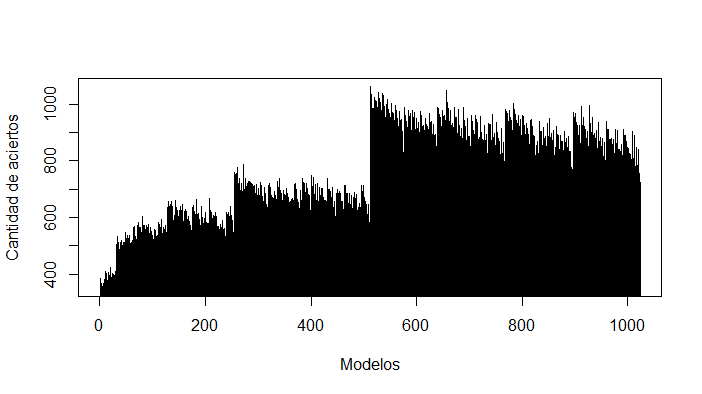
\includegraphics[width=0.5\textwidth]{histograma}
\caption{Histograma de frecuencia absoluta de aciertos de los $1023$ modelos en toda la base.}
\label{histograma}
\end{figure}

Con toda esta nueva información obtenida y el cambio de paradigma propuesto, nuestros siguientes pasos fueron aplicar algoritmos de aprendizaje automático para buscar la relación entre el ensamble de estimaciones de precios y el precio correcto. Para esto utilizamos Métodos de Ensamble de Modelos, Bagging basado en Árboles de Decisión y Redes Neuronales.

Una forma intuitiva, que nos ayudó en la visualización de este problema, fue la de considerar al Ensamble de Modelos por Modelos Lineales ajustados mediante la ventana móvil y su correspondientes estimaciones de precios como un conjunto de expertos y sus respectivas opiniones sobre el futuro precio. Hemos mostrado previamente que en este conjunto de expertos, entre sus opiniones hay un alto porcentaje de acierto ($76.15\%$). 

Un primer criterio para sintetizar estas opiniones es el algoritmo de Ensamble de Modelos, donde se promedian las opiniones buscando mediar las  más extremas y lograr un consenso. En la Figura \ref{diagramExpertMean} se muestra el procedimiento, donde para cada momento $n$ a predecir de la muestra de testeo se realiza una ventana de $25$ rezagos, se obtienen las $1023$ predicciones para el precio del momento $n$ (opiniones expertas) y se promedian para obtener el precio estimado. Luego se calcula el RMSE prediciendo una a una las muestras de testeo y se compara con el precio correcto.

\begin{figure}[!hbt]
\centering
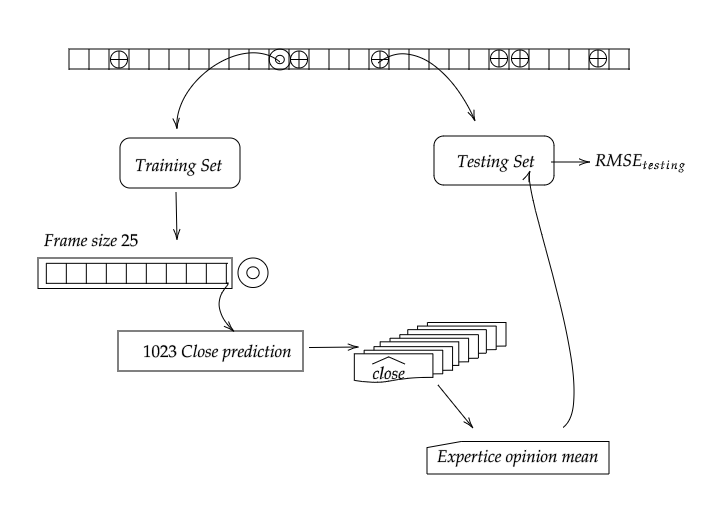
\includegraphics[width=0.5\textwidth]{diagramExpertMean}
\caption{Diagrama de Ensamble de Modelos donde para la predicción del momento $n$ se genera una ventana de $25$ rezagos y se ajustan $1023$ modelos de los cuales sus predicciones, consideradas como opiniones expertas, se promedian para obtener un consenso. Para obtener el RMSE se predicen una a una las muestras de testeo y se comparan con el precio correcto.}
\label{diagramExpertMean}
\end{figure}

El segundo criterio utilizado para buscar la relación entre el ensamble de precios estimados por ventanas móviles y el precio correcto fue el de utilizar el algoritmo de Bagging con Árboles de Regresión. Este algoritmo más flexible fue seleccionado con la intención de lograr capturar en su complejidad de decisión el problema que representa sintetizar estas $1023$ opiniones expertas y sus posibles relaciones con el precio correcto.

El método de Bagging con Árboles de Regresión se ajusta con exactamente la misma muestra de entrenamiento con la que se realizó la primera estimación por Modelos Lineales pero esta vez las variables son el ensamble de $1023$ predicciones. Una vez obtenido mediante Bagging el modelo ajustado, se predice con este modelo cada una de las muestras de testeo y se calcula el RMSE. En la Figura \ref{diagramBagging} se sintetiza este algoritmo.

\begin{figure}[!hbt]
\centering
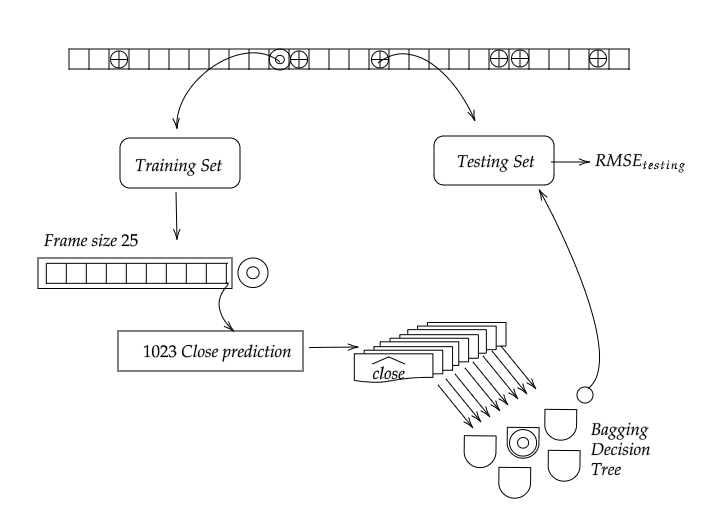
\includegraphics[width=0.5\textwidth]{diagramBagging}
\caption{Diagrama de Bagging por Árboles de Decisión donde se ajusta un modelo a partir de la nueva base generada, siendo las variables que entrenan este modelo las $1023$ predicciones que representan opiniones de expertos. Para obtener el RMSE se utilizan las predicciones del modelo obtenido con la muestra de testeo.}
\label{diagramBagging}
\end{figure}

El tercer criterio cumple el mismo procedimiento que el algoritmo anterior, pero esta vez aplicado a Redes Neuronales. Primero se entrena una red donde sus variables de entrada son el ensamble de $1023$ opiniones de expertos generados por una ventana de $25$ rezagos para cada momento $n$ de la muestra de entrenamiento original y posteriormente se calcula el RMSE con el modelo obtenido sobre la muestra de testeo. En la Figura \ref{diagramNeuralNetwork} se sintetiza este algoritmo.

\begin{figure}[!hbt]
\centering
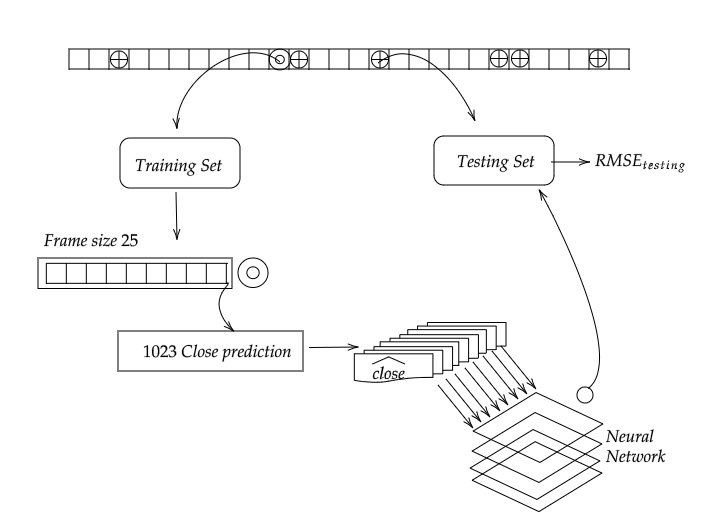
\includegraphics[width=0.5\textwidth]{diagramNeuralNetwork}
\caption{Diagrama de Redes Neuronales donde se ajusta un modelo a partir de la nueva base generada, siendo las variables de entrada que entrenan este modelo las $1023$ predicciones que representan opiniones de expertos. Para obtener el RMSE se utilizan las predicciones obtenidas con la Red Neuronal desde la muestra de testeo.}
\label{diagramNeuralNetwork}
\end{figure}


\section{Resultados}

El objetivo de esta investigación es encontrar metodologías alternativas a investigaciones previas y la literatura existente sobre la predicción del precio de $Cierre$ del Bitcoin y lograr mejorar el rendimiento propuesto. 

Para establecer un marco de comparación primariamente ajustamos un modelo mediante Regresión Lineal dividiendo la base de datos aleatoriamente en un $70\%$ de entrenamiento y un $30\%$ de testeo. En este caso el modelo con el mejor ajuste mediante las variables obtenidas a partir de cinco rezagos de $Cierre$ y $Volumen$ del precio del Bitcoin, logra un RMSE de predicción de  $231.4537$, este modelo está compuesto por dos variables explicativas, $closeLag1$ y $closeLag3$, que representan el primer y tercer rezago del precio de $Cierre$, respectivamente. Si bien en investigaciones previas utilizando la misma técnica, pero con bases de datos en distintos momentos del tiempo, el modelo con mejor ajuste seleccionado difiere del elegido en esta investigación, el RMSE alcanzado refleja un mismo rendimiento de predicción.

El primer algoritmo propuesto es el de Ensamble de Modelos. El RMSE resultante es de $91.33031$ con respecto a las observaciones de la muestra de testeo original. Esta propuesta ya logra duplicar el rendimiento obtenido por el RMSE de referencia obtenido mediante Modelos Lineales. 


El segundo algoritmo utilizado es el de Bagging con Árboles de Regresión. Para esta técnica se utilizó el paquete randomForest~\cite{randomForest} de R~\cite{r}. Este algoritmo refleja mayor flexibilidad de ajuste en las predicciones. El RMSE resultante es de $78.87432$ con respecto a las observaciones de testeo de la muestra original. Este modelo fue obtenido utilizando $100$ árboles y $1023$ variables de entrada correspondientes al ensamble de $1023$ predicciones por ventanas móviles para cada muestra. En la Figura \ref{aciertoBagging} se contrastan las $12$ variables explicativas utilizadas para Bagging que tienen más peso en la media de precisión en las predicciones en la muestra cuando cada una de estas se excluye del modelo con el histograma de frecuencia absoluta de aciertos de los $1023$ modelos. Podemos ver que la mayoría de estas variables se encuentran sobre el tercer umbral previamente mencionado.

\begin{figure}[!hbt]
\centering
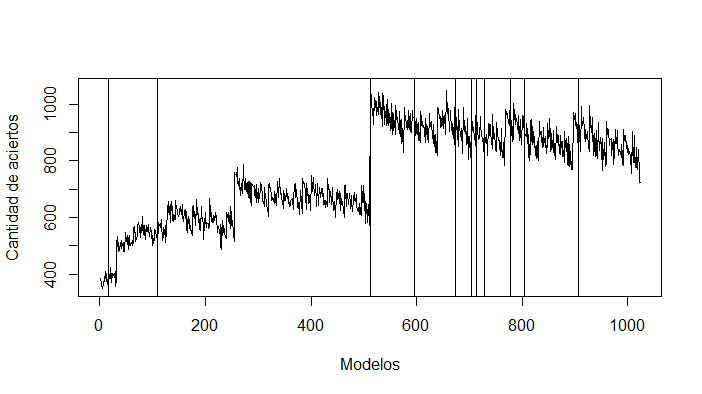
\includegraphics[width=0.5\textwidth]{aciertoBagging}
\caption{Histograma de frecuencia absoluta de aciertos de los $1023$ modelos en toda la base. En líneas verticales se muestran las $12$ variables explicativas utilizadas para Bagging que tienen más peso en la media de precisión en las predicciones cuando cada una de estas se excluye del modelo.}
\label{aciertoBagging}
\end{figure}

En la Figura \ref{errorMSEBagging} se muestra como disminuye el error MSE a medida que se aumenta la cantidad de árboles utilizada para Bagging, esto concuerda con la hipótesis inicial planteada que mayor complejidad de decisión obtiene un mejor rendimiento del modelo.

\begin{figure}[!hbt]
\centering
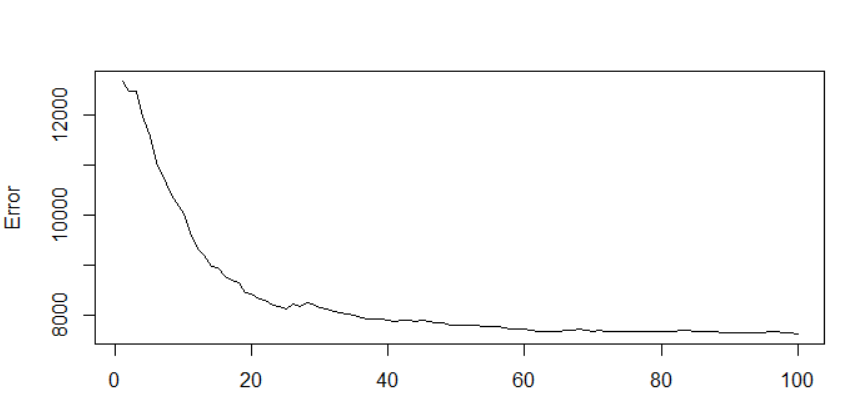
\includegraphics[width=0.5\textwidth]{errorMSEBagging}
\caption{Error MSE de Bagging a medida que aumenta la cantidad de árboles empleados.}
\label{errorMSEBagging}
\end{figure}

Este algoritmo es el que logra el mejor RMSE de todas las propuestas.

El tercer algoritmo implementado son las Redes Neuronales, que según la configuración de nodos, capas y funciones de activación, puede ser el algoritmo con mayor flexibilidad y complejidad de decisión. Asimismo, el costo computacional requerido es exponencial. Para esta investigación se utilizó una Red Neuronal con $1023$ variables de entrada, tres capas ocultas, donde la primera capa oculta es utilizada para la estandarización de los valores de las variables de entrada y las siguientes dos capas están compuestas por 16 y 8 nodos respectivamente, una capa de salida y funciones de activación relu. Fue necesario un entrenamiento de $1000$ épocas para lograr un ajuste satisfactorio. El RMSE que logra esta red con respecto a la muestra original de testeo es de $136.8908$. 

Se utilizó el paquete Keras~\cite{keras} de R~\cite{r} que es una capa de alto nivel de Tensorflow~\cite{tensorflow}. Tensorflow es una biblioteca de código abierto propiedad de Google y de las más utilizadas actualmente para el aprendizaje profundo.

En el Cuadro \ref{redesModelTuning} se muestra la comparación de las dos configuraciones experimentadas en esta investigación para Redes Neuronales. Se puede observar que el rendimiento con menor cantidad de nodos en las capas afecta enormemente de forma negativa el rendimiento de la red.

De todos los algoritmos propuestos en esta investigación, las Redes Neuronales son las que logran un peor desempeño, pero asimismo logran superar ampliamente el rendimiento alcanzado por el modelo de referencia generado por Modelos Lineales y deja las puertas abiertas a múltiples configuraciones más complejas para mejorar su poder de predicción. Realizar esto dentro de esta investigación exigía un poder computacional fuera del alcance técnico empleado. 

\begin{table}[!hbt]
\centering
\caption{Cantidad de nodos por capa utilizados para entrenar las Redes Neuronales para la predicción del $Cierre$ de Bitcoin y el RMSE obtenido con respecto a la muestra de testeo original. Todas las capas tienen una función de activación relu.}
\label{redesModelTuning}
\begingroup\setlength{\fboxsep}{0pt}
\colorbox{lightgray}{%
\begin{tabular}{|l|l|l|l|}
\hline Capa 2 &  Capa 3  &  Activación & RMSE \\
\hline 16 & 8  &  relu &136.8908\\
\hline 8 & 8  &  relu &10640.92\\
\hline
\end{tabular}%
}\endgroup
\end{table}

En el Cuadro~\ref{RMSEFinal} se muestra el desempeño de cada uno de los modelos seleccionados, Ensamble de Modelos, Bagging y Redes Neuronales, comparados con los resultados obtenidos por el modelo de referencia basado en Modelos Lineales. En este caso el modelo ajustado por Bagging es el que logra mejores resultados. Asimismo, se puede observar que los tres modelos propuestos superan el rendimiento del modelo de referencia original.

\begin{table}[!hbt]
\centering
\caption{Mejores resultados de RMSE obtenidos para las cuatro técnicas utilizadas en la predicción del $Cierre$ de Bitcoin. }
\label{RMSEFinal}
\begingroup\setlength{\fboxsep}{0pt}
\colorbox{lightgray}{%
\begin{tabular}{|l|l|}
\hline Algoritmo de predicción & RMSE \\
\hline Modelos Lineales & 231.4537\\
\hline Ensamble de Modelos & 91.33031\\
\hline Bagging (Árbol de Decisión)& 78.87432\\
\hline Redes Neuronales & 136.8908 \\
\hline
\end{tabular}%
}\endgroup
\end{table}


\section{Conclusiones}

El objetivo de esta investigación fue buscar un modelo alternativo a las técnicas propuestas por la literatura e investigaciones recientes para la predicción del precio del Bitcoin que logre mejorar los rendimientos alcanzados en estas. Para esto se presentó un sistema de ventanas móviles el cual genera un ensamble de estimadores mediante Modelos Lineales, que son consideradas como opiniones expertas, y se utilizaron diversas técnicas para sintetizar estas opiniones en una predicción. Los resultados obtenidos muestran que bajo esta perspectiva, la técnica de Bagging obtiene un rendimiento ampliamente mayor que los modelos propuestos originalmente.

Asimismo, se entrevé que la flexibilización y el aumento de la complejidad del sistema de predicción para este enfoque es el camino correcto. La tendencia mostrada indica que posibles modelos con más árboles pueden lograr mejores rendimientos y deja las puertas abiertas a futuras experimentaciones con Redes Neuronales con arquitecturas más complejas, ya que si bien las Redes Neuronales no fueron el algoritmo que logró un mejor rendimiento entre los propuestos, si mostró una tendencia a la mejora en predicción a medida que se aumentaba la complejidad de estas redes. 

De este modo, el nuevo enfoque presentado en esta investigación aplicado al algoritmo de Bagging sobre Árboles de Regresión se convierte en la opción candidata para la predicción del precio del Bitcoin.



          
%
\begin{thebibliography}{99}

\bibitem{Bitcoin_revolucion_monetaria}
Sangoi, F.
{\em Bitcoin. ¿Una revolución monetaria?}
Universidad de Buenos Aires.
%
\bibitem{regression_for_bitcoin_price}
Azim Muhammad Fahmi, Noor Azah Samsudin, Aida Mustapha, 
Nazim Razali, Shamsul Kamal Ahmad Khalid. (2018).
{\em Regression based Analysis for Bitcoin Price Prediction.}
Faculty of Computer Science and Information Technology, Universiti Tun Hussein Onn Malaysia.

\bibitem{Satoshi}
Nakamoto, S. (2008).
{\em Bitcoin: A Peer-to-Peer Electronic Cash System.}

\bibitem{Blockchain}
Carlos Dolader Retmal et al.
{\em La blockchain: fundamentos, aplicaciones y relación con otras tecnologías disruptivas}, Universitat Politécnica de Catalunya.

\bibitem{Blockchain_science}
Karame, G., Huth, M., Vishik, C. (2020).
{\em An overview of blockchain science and
engineering.} R. Soc. Open Sci. 7: 200168.
http://dx.doi.org/10.1098/rsos.200168


\bibitem{Bayesian}
Shah, D., Zhang, K. (2014).
{\em Bayesian regression and Bitcoin.} 
Laboratory for Information and Decision Systems
Department of EECS, Massachusetts Institute of Technology.


\bibitem{Methods}
Ferdiansyah, Siti Hajar Othmanb, Raja Zahilah Raja Md Radzic, Deris Stiawan. (2019).
{\em A Study of Bitcoin Stock Market Prediction: Methods, Techniques and Tools.} 

\bibitem{Bitcoin_bubbles_predictable}
Wheatley, S., Sornette, D., Huber, T., Reppen, M., Gantner, RN. (2019). 
{\em Are Bitcoin bubbles predictable? Combining a generalized
Metcalfe’s Law and the Log-Periodic Power Law
Singularity model.} R. Soc. open sci. 6: 180538.
http://dx.doi.org/10.1098/rsos.180538

\bibitem{forecastinBitcoinClosing}
Uras, N., Marchesi, L., Marchesi, M., Tonelli, R. (2020)
{\em Forecasting Bitcoin closing price series using linear
regression and neural networks models}. Department of Mathematics and Computer Science, University of Cagliari.

\bibitem{forecast_bitcoin_GAM}
Asante Gyamerah, S. (2020).
{\em On forecasting the intraday Bitcoin price using ensemble of variational
mode decomposition and generalized additive model}. Pan African University, Institute for Basic Sciences, Technology, and Innovation.
https://doi.org/10.1016/
j.jksuci.2020.01.006


\bibitem{bitcoin_ML}
McNally, S. (2016).
{\em Predicting the price of Bitcoin using Machine Learning.} School of Computing National College of Ireland.

\bibitem{mainDriversBitcoin}
Kristoufek, L. (2015). {\em What Are the Main
Drivers of the Bitcoin Price? Evidence from Wavelet
Coherence Analysis.} PLoS ONE 10(4): e0123923.
doi:10.1371/journal.pone.0123923

\bibitem{bitcoin_ML_PSA}
Rajua, S., Mohammad, A. (2020).
{\em Real-Time Prediction of BITCOIN Price using Machine Learning Techniques and Public Sentiment Analysis.}
Computer Science, International Islamic University Malaysia.

\bibitem{bitcoin_socialmedia}
Burnie, A., Yilmaz, E. (2019). 
{\em Social media and bitcoin metrics: which words matter.}
R. Soc. open sci. 6: 191068.
http://dx.doi.org/10.1098/rsos.191068

\bibitem{bitcoin_socialmedia}
Garcia, D., Schweitzer, F. (2015).
{\em Social signals and algorithmic trading of Bitcoin.} R. Soc. open sci. 2: 150288.
http://dx.doi.org/10.1098/rsos.150288

\bibitem{Predictor_Impact_Web_Search_Media__Bitcoin_Trading_Volumes}
Matta, M.; Lunesu, I. and Marchesi, M.  (2015).
{\em The Predictor Impact of Web Search Media On Bitcoin Trading Volumes.}
Universita’ degli Studi di Cagliari.

\bibitem{Bitcoin_variables}
Hakim, R. (2020)
{\em Bitcoin pricing: impact of attractiveness variables.}
Sao Paulo School Of Economics.
https://doi.org/10.1186/s40854-020-00176-3

\bibitem{r}
R Core Team. (2020). 
{\em R: A Language and Environment for Statistical Computing.}
Vienna, Austria: R Foundation for Statistical Computing. 
https://www.R-project.org/

\bibitem{tree}
Ripley, B. (2019). 
{\em tree: Classification and Regression Trees.}
https://CRAN.R-project.org/package=tree

\bibitem{randomForest}
Liaw, A., Wiener, M. (2002). 
{\em Classification and Regression by randomForest.}
https://CRAN.R-project.org/doc/Rnews/

\bibitem{keras}
Allaire, JJ., Chollet, F. (2020).
{\em keras: R Interface to 'Keras'.}
https://CRAN.R-project.org/package=keras

\bibitem{tfdatasets}
Allaire, JJ., Tang, Y., Ushey, K. (2020).
{\em tfdatasets: Interface to 'TensorFlow' Datasets.}
https://CRAN.R-project.org/package=tfdatasets

\bibitem{tfruns}
Allaire, JJ. (2018).
{\em tfruns: Training Run Tools for 'TensorFlow'.}
https://CRAN.R-project.org/package=tfruns

\bibitem{tensorflow}
Allaire, JJ., Tang, Y. (2020).
{\em tensorflow: R Interface to 'TensorFlow'.}
https://CRAN.R-project.org/package=tensorflow

\bibitem{libroCurso}
Gareth, J., Witten, D., Hastie, T., Tibshirani, R. (2013). 
{\em An introduction to statistical learning : with applications in R.}
New York: Springer.

\bibitem{libroCurso2}
Hastie, T., Tibshirani, R., Friedman, J. (2017). 
{\em The Elements of Statistical Learning: Data Mining, Inference, and Prediction.}
New York: Springer, 2nd edition.

\bibitem{paper1}
Alcalde, V., Martinez Angerosa, P. (2020). 
{\em Predicción del precio diario de Cierre y dirección del Bitcoin mediante Modelos de Regresión Lineal Múltiple y Logísticos.}

\bibitem{paper2}
Alcalde, V., Martinez Angerosa, P. (2020). 
{\em Predicción del precio diario de Cierre del
Bitcoin mediante Bagging, Árboles de
decisión y Redes Neuronales.}

\bibitem{Goodfellow}
Goodfellow, I., Bengio, Y., Courville, A. (2016). 
{\em Deep Learning.} MIT Press. 
http://www.deeplearningbook.org


\end{thebibliography}
\end{document}
